\documentclass[12pt,lot,lof]{puthesis_undergraduate}
\usepackage{amsfonts}
\usepackage{amssymb}
\usepackage{amsmath}
\usepackage{amsthm}
\usepackage{latexsym}
\usepackage{graphicx}
%\usepackage{setspace}
\usepackage{textcomp}
\usepackage[round, longnamesfirst]{natbib} % for nice bibliography

%%%%%% ENVIRONMENTS %%%%%%
%\swapnumbers
%\newtheorem{theorem}{Theorem}
%\newtheorem{proposition}[theorem]{Proposition}
%\newtheorem{lemma}[theorem]{Lemma}
%\newtheorem{definition}[theorem]{Definition}
%\newtheorem{corollary}[theorem]{Corollary}
%\newtheorem{remark}[theorem]{Remark}
%\newtheorem{conjecture}[theorem]{Conjecture}
%\newtheorem{notation}[theorem]{Notation}
%\newtheorem{example}[theorem]{Example}
%\newtheorem{exercise}{Exercise}
%\newtheorem*{notes}{Notes}

% For PUthesis.cls use the following definitions:
\newtheorem{theorem}{Theorem}[section]
\newtheorem{lemma}[theorem]{Lemma}
\newtheorem{corollary}[theorem]{Corollary}
\newtheorem{proposition}[theorem]{Proposition}
\newtheorem{definition}[theorem]{Definition}
\newtheorem{claim}{Claim}
\newtheorem{conjecture}[theorem]{Conjecture}
\newtheorem{observation}[theorem]{Observation}
\newtheorem{problem}[theorem]{Problem}



%%%%%% NEW COMMANDS/OPERATORS %%%%%%
\DeclareMathOperator{\esup}{\text{ess\;sup}}
\providecommand{\abs}[1]{\lvert#1\rvert} % absolute value function
\renewcommand{\P}{\mathbb{P}}  % probability measure
\renewcommand{\O}{\mathcal{O}} % order notation
\newcommand{\PP}{\P^\star} % pricing probability measure
\newcommand{\E}{\mathbb{E}}  % expectation
\newcommand{\Var}{\mathrm{Var}}
\newcommand{\EE}{\E^\star}   % expectation under the pricing measure
\newcommand{\V}{\text{Var}} % variance
\newcommand{\F}{\mathcal{F}} % filtration
\newcommand{\G}{\mathcal{G}} % filtration
\renewcommand{\H}{\mathcal{H}} % filtration
\newcommand{\Fb}{\mathbb{F}} % filtration
\newcommand{\N}{\mathbb{N}}  % integers
\newcommand{\R}{\mathbb{R}}  % real numbers
%\renewcommand{\C}{\mathbb{C}}  % complex numbers
\newcommand{\argmin}{\mathop{\mathrm{arg\,min}}} % arg min operator
\newcommand{\cpb}{c^{\mbox{\scriptsize pb}}} % protection buyer payment
\newcommand{\cps}{c^{\mbox{\scriptsize ps}}} % protection seller payment
\newcommand{\cds}{c^{\mbox{\scriptsize ds}}} % CDS spread

\newcommand{\T}{\mathcal{T}} % tenor
\renewcommand{\vec}[1]{\mbox{\boldmath $#1$}} % boldface 1 for the indicator function
\newcommand{\ind}{\vec{1}}                    % boldface 1 for the indicator function
\newcommand{\Ws}{W^\star_t}
\newcommand{\tWs}{\widetilde{W}^\star_t}
\newcommand{\tWz}{\widetilde{W}^0_t}
\newcommand{\tW}{\widetilde{W}}

%%%%%% Shortcut expressions %%%%%%
\newcommand{\pb}{protection buyer}
\newcommand{\ps}{protection seller}
\newcommand{\BibTeX}{{\sc Bib}\TeX}

%%%%%% Greeks %%%%%%
\newcommand{\eps}{\varepsilon}
\newcommand{\de}{\delta}
\newcommand{\fee}{\varphi}
\newcommand{\half}{\frac{1}{2}}

%%%%%% PDEs %%%%%%%
\newcommand{\pa}{\partial}
\renewcommand{\L}{\mathcal{L}}
\newcommand{\M}{\mathcal{M}}
\newcommand{\A}{\mathcal{A}}
\newcommand{\wA}{\widetilde{\A}}
\newcommand{\wlop}{\widetilde{\L}}
\newcommand{\wmop}{\widetilde{\M}}
\newcommand{\lbs}{\L_{BS}}
\newcommand{\lbss}{\L_{BS^\star}}
\newcommand{\lzero}{\L_{0}}
\newcommand{\lone}{\L_{1}}
\newcommand{\ltwo}{\L_{2}}
\newcommand{\wled}{\widetilde{\L}^{\eps,\de}}
\newcommand{\wlone}{\widetilde{\L}_1}
\newcommand{\wltwo}{\widetilde{\L}_2}
\newcommand{\cltwo}{\langle \L_2 \rangle}
\newcommand{\cwltwo}{\left\langle \wltwo \right\rangle}
\newcommand{\mone}{\M_{1}}
\newcommand{\mtwo}{\M_{2}}
\newcommand{\mthree}{\M_{3}}
\newcommand{\wmone}{\widetilde{\M}_1}
\newcommand{\fc}{\langle f \rangle}  % <f>

\newcommand{\bes}{\begin{equation*}}

%%%%%% OLD ONES %%%%%%
%\newcommand{\sigbar}{\overline{\sigma}}
%\newcommand{\sigstar}{\sigma_\star}
%\newcommand{\CBS}{C_{BS}}
%\newcommand{\CBSs}{C_{BS^\star}}
%\newcommand{\BS}{Black-Scholes }
%\newcommand{\vol}{volatility}
%\newcommand{\SV}{stochastic volatility }
%\newcommand{\PP}{{\mathord{I\kern -.33em P}}}
%\newcommand{\EE}{{\mathord{I\kern -.33em E}}}
%\newcommand{\RR}{{\mathord{I\kern -.33em R}}}
%\newcommand{\1}{{\mathord{1\kern -.26em \text{I}}}}
%\newcommand{\calp}{{\PP}}
%\newcommand{\EEE}{{\EE^{\star}}}
%\newcommand{\PPP}{{\PP^{\star}}}
%\newcommand{\ssb}{\overline{\sigma^2}}


%Do not un-comment the next two lines
%Included for Gather Purpose only in WinEdt (ignore for other editors):
%input "./Bibliography/refs.bib"

\title{Visualizing United State's Traffic Flow}
\submitted{12 May 2015}  %graduation date
\author{Tharald S. Fongaard \& Jacob Perricone}
\advisor{Professor Alain Kornhauser} %
\dedication{To The Hereditary Kingdom of Norway}


\abstract{
By analyzing trip generation in the United States, we will display key statistics in an informative graphic user interface. Specifically, given a node network of the entire nation and trip generation files, we will provide a means to determine the number of vehicles, people, and the average vehicle occupancy on each link at each time throughout 
the day. 

}

\acknowledgements{
Here are the acknowledgments. I'm sure you know what to do
here\ldots thanks, and thanks!

}

\begin{document}
\chapter{Introduction}\label{ch:intro}  %insert chapter title
This is the introduction of my sample thesis. Let me just state that
this is a very, very limited introduction to \LaTeX, and I can not
do justice to it through the next few pages.

I recommend reading this .pdf file along with the .tex file open on
the side so that you can compare the pure ASCII text and the final
result after compilation.

\section{A Different Word Processing System} \label{ch:anotherintro}
I highly recommend the booklet ``The Not So Short Introduction to
\LaTeXe{}'' which is free and very well-written. It is available on:
\begin{center}
\verb|http://tobi.oetiker.ch/lshort/lshort.pdf|.
\end{center}

\noindent I refer you to the introduction there.
 % and path to the .tex file (no need to include .tex)

\chapter{Development of the Department of Operations Research and Financial Engineering}  %continue adding chapter titles
%%% This is the development.tex

This Chapter has purposefully a very long title to illustrate how
\LaTeXe{} handles such long names. Now it is a good time to look on
the table of contents and see how this Chapter and also
Chapter~\ref{ch:intro} are listed. Notice that the number 1 in the
phrase ``and also Chapter 1'' is automatically generated by using
the command \verb|\ref{ch:intro}|, because we labeled
Chapter~\ref{ch:intro} `\verb|ch:intro|' by using the command
\verb|\label{ch:intro}| after the \verb|\chapter{Introduction}|
declaration.

\section{Initial Setup}
A few things here to start. And here as well, since we need to fill
in at least a line. Almost\ldots, there we go!

Notice that I entered ellipses after the word `Almost' above with
the command \verb|\ldots|, and not by simply typing three dots.
Compare the result here: \ldots vs. ...\footnote{Word does that too,
but lousily!}

Maybe some more words in a new paragraph. And more, and more, and
more. Furthermore, additionally, in addition, and so on. Notice here
that the word `Furthermore' was broken into `Fur-' and `thermore' in
order to fit the line---Word, as stupid as it is, would simply place
the entire word on the next line, thus increasing the distance
between words on the first line to fill up the entire line.

\subsection{Additional Structure: The Use of Subsections}
\label{sec:structure} We are in a subsection now (two levels down
from a Chapter). When we refer to $X.Y.Z$, we mean Chapter $X$,
Section $Y$, and subsection $Z$. We declare a Chapter by the command
\verb|\chapter{|\emph{title of Chapter}\verb|}|, a Section by
\verb|\section{|\emph{title of Section}\verb|}|, and so on.

The nice thing about \LaTeX{} is that it takes care of the chapter,
section, and subsection numbering automatically. If I were to add
another subsection before this one the subsection number would
change (increment by one). This section is \ref{sec:structure} and I
referred to it using the command \verb|\ref{|\emph{label of this
section}\verb|}|. I inserted a label right after the
\verb|\subsection| declaration by typing \verb|\label{|\emph{label
of this section}\verb|}|.

\subsubsection{A subsubsection}\label{subsub} Just for fun! Notice
that no number is alloted for such a low level environment but it
sometimes useful.

\subsection{Another Subsection}
And so on\ldots.

\section{Mathematical Symbols}
Let $X=\{X_n, n\in \N\}$ be a Markov chain with state space
$\mathcal{D}$. Throughout this thesis, we use the notation
\begin{equation}
p_{ij} := \P\{X_{n+1} = j \mid X_n = i\}, \quad i,j \in \mathcal{D}
\label{pij}
\end{equation}
for the transition probabilities of the Markov chain $X$.
Furthermore, we denote by $P$ the transition matrix, $P =
[p_{ij}]_{i,j\in\mathcal{D}}$.

When we wrote \eqref{pij} we implicitly assumed that the Markov
chain $X$ is time-homogeneous.

Let us also define $Y$,
\begin{equation*}
Y = (Y_n)_{n = 0,1,2,\ldots}
\end{equation*}
to be another process. Notice that the second equation does not take
a number on the right---this is the use of \verb|\begin{equation*}|
environment.

Notice that the all the math characters, $X$, $\mathcal{D}$, and
others such as $\alpha, \beta, \gamma$ are part of the text in
\LaTeX{}. On the contrary, Word includes such characters as foreign
objects (usually images), which increases the size of the document
file, sometimes makes them disappear, but most importantly are not
as aesthetically pleasing as the resulting characters here.

\section{Citing and Bibliography}
When working with large documents you need an easy way to cite your
references without having to go back to your list all the time to
remember the names of the authors and the year of publication. Even
more importantly, you need to have all your references listed in the
end of the document in alphabetical order. Of course, they all need
to be syntactically the same so that alone makes the manual entry of
references a big pain. Thankfully, \LaTeX{} takes care of that in a
very easy and elegant way, using \BibTeX.

I cite here a few books, papers, and technical reports, and please
go to page \pageref{bib} to see the resulting bibliography.

According to the books by \cite{C75}, \cite{BR02}, and \cite{MR97}
and the articles by \cite{DG01}, \cite{BBM05}, and \cite{CFPS04} we
conclude absolutely nothing. However, in his report, \cite{A04}
claims that otherwise. All these citations were entered by \verb|\cite{|\emph{citation label}\verb|}|.
 
Notice the different citation style that follows: it is parenthetical, and observe that only one pair of parentheses is required \cite[see Theorem 5.2][pg. 32]{AMM05}. This citation is entered by typing \verb|\cite[see Theorem 5.2][pg. 32]{AMM05}| in the \verb|.tex| file. (Here, the citation label corresponding to \cite{AMM05} is obviously \verb|AMM05|.)


The citations are included in the file \verb|refs.bib| under the
folder \verb|Bibliography|. You can modify it and make your own
references. I highly recommend using \emph{JabRef} for managing your bibliography entries, because it makes it a piece of cake to do a lot of \emph{dirty} work. \emph{JabRef} is free and it works as a Java Application.

Also notice that \LaTeX{}, by default, includes in the Bibliography section only the references you actually cited throughout the text. If you want a source to appear in the Bibliography section without actually citing it anywhere in your text use the command \verb|\nocite{|\emph{citation label}\verb|}|. For example here I type \verb|\nocite{B95}| \nocite{B95} and you see no citation appear---however look at the fourth entry of the Bibliography. That cited book does not appear anywhere in this thesis, other than the Bibliography.

\section{Referencing Figures and Tables}
The very informative Figure~\ref{fig:dens} is on page~\pageref{fig:dens}. Both of these numbers were automatically generated---which is great when you add a new figure before the one you just inserted, because the numbering changes automatically for you. Use \verb|\ref{fig:dens}| for the figure number and \verb|\pageref{fig:dens}| for the page number where the figure is located. Here, \verb|fig:dens| was the label of the figure (see actual \verb|.tex| file for more information). Remember that \LaTeX{} does not work like Word---the figures and tables are \textbf{not} always placed exactly where you want them, so avoid writing ``according to the figure below\ldots,'' and prefer writing ``according to Figure~[\emph{figure number}]\ldots,'' instead. The same things go unchanged for tables. Notice that when I talk about figures and tables in general, I do not need to capitalize them, however if I talk specifically about Figure~\ref{fig:dens} and Table~\ref{tab:cdo}, I'd better respect them and capitalize the `f' and the `t.'

Since we're at it, notice that the quotes `, ', ``, '' are not inserted like in Word. For ` you need to use the \verb|`| key that is located above the \verb|Tab| button. For ' you just press the \verb|'| key, exactly to the left of the \verb|Enter| key. For double quotes just double the appropriate single quotes without leaving any space.


\chapter{Analysis of Problem}
%% This is the analysis.tex file

Time for some analysis, and probably graphs and tables. Thankfully
\LaTeX{} (and \LaTeXe{}) provides very nice environments for both.

\section{Preliminary Analysis}
\begin{figure}[t]
\begin{center}
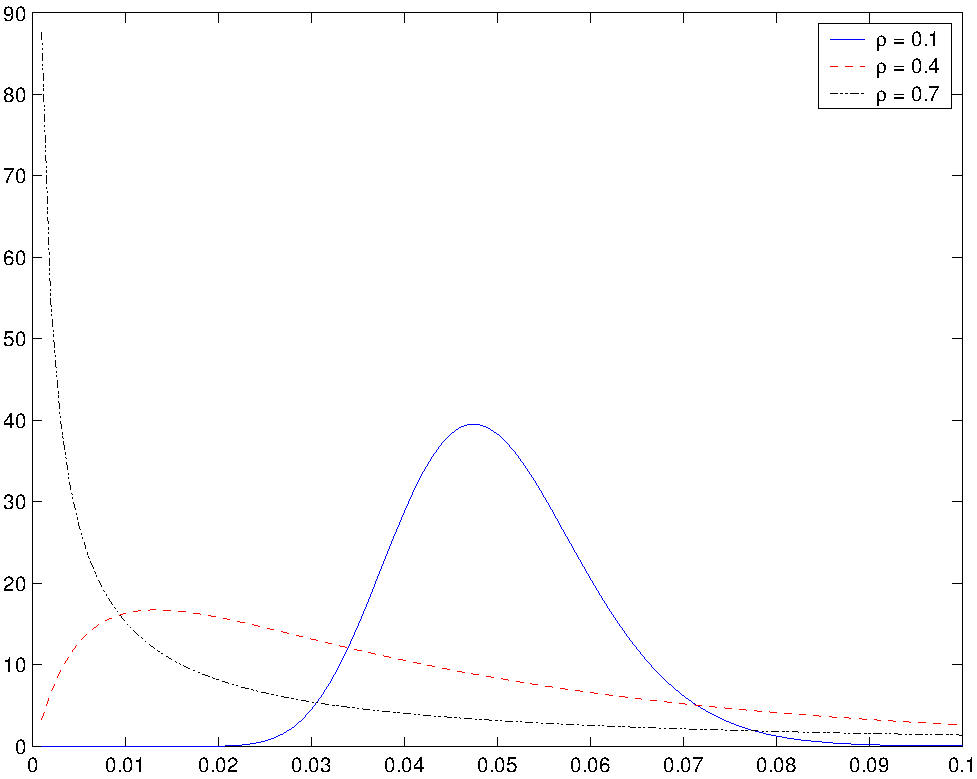
\includegraphics[width=0.8\textwidth]{./Figures/dens.pdf}
\caption{The density function $f$ as given in \eqref{density} for
  three different $\rho$'s and $\bar{p} = 0.05$. (Plotted on $[0,
  0.1]$ for convenience.)}
\label{fig:dens}
\end{center}
\end{figure}
Assume that the random variable $D$ given $\tilde{p} = p$ is
binomially distributed with parameters 50 and $p$ (probability of
success, in this case default). We also take the cumulative
distribution function of $\tilde{p}$ to be
\begin{equation*}
F(\theta) = \P\{\tilde{p} \le \theta\} = \Phi \left( \frac{1}{\rho}
\left(\sqrt{1 - \rho^2}\, \Phi^{-1}(\theta) - \Phi^{-1}(\bar{p})
\right) \right)
\end{equation*}
where $\Phi$ is the cumulative standard normal distribution
function, $\rho$ is the correlation coefficient between the
idiosyncratic and market factors and $\bar{p}$ is the mean default
probability ($\bar{p} = \E \tilde{p}$). To calculate the density of
$\tilde{p}$ let
\begin{eqnarray*}
h(\theta, \rho, \bar{p}) &:=& \frac{1}{\rho} \left(\sqrt{1 -
\rho^2}\, \Phi^{-1}(\theta) - \Phi^{-1}(\bar{p}) \right), \\
\varphi(\theta) &:=& \frac{d}{d \theta} \Phi(\theta) =
\frac{1}{\sqrt{2 \pi}} e^{- \theta^2/2},
\end{eqnarray*}
and notice that since $\Phi$ is a bijection we have
\[\Phi \circ \Phi^{-1}(\theta) = \Phi^{-1} \circ \Phi(\theta) =
\theta, \] for every $\theta \in \R$. Then, we have for the density
of $\tilde{p}$,
\begin{eqnarray}
f(\theta, \rho, \bar{p}) &=& \frac{d}{d \theta} F(\theta) =
\Phi'(h(\theta, \rho, \bar{p})) \frac{\pa}{\pa \theta} h(\theta,
\rho, \bar{p}) \nonumber \\
&=& \varphi(h(\theta, \rho, \bar{p})) \frac{\sqrt{1 -
\rho^2}}{\rho} \frac{d}{d \theta} \Phi^{-1}(\theta) \nonumber \\
&=& \varphi(h(\theta, \rho, \bar{p})) \frac{\sqrt{1 - \rho^2}}{\rho}
\frac{1}{\varphi (\Phi^{-1}(\theta))}, \label{density}
\end{eqnarray}
for $\theta \in (0,1)$ and zero otherwise, since
\begin{eqnarray*}
\frac{d}{d \theta} \left(\Phi (\Phi^{-1}(\theta)) \right) &=&
\Phi'(\Phi^{-1}(\theta)) \frac{d}{d \theta} \Phi^{-1}(\theta)
\Leftrightarrow \\
\frac{d}{d \theta} \theta &=& \varphi(\Phi^{-1}(\theta))
\frac{d}{d \theta} \Phi^{-1}(\theta) \Leftrightarrow \\
\frac{d}{d \theta} \Phi^{-1}(\theta) &=&
\frac{1}{\varphi(\Phi^{-1}(\theta))}.
\end{eqnarray*}



The density of $\tilde{p}$ is shown in Figure \ref{fig:dens} for
three different values of $\rho$ and $\bar{p} = 0.05$. The effect of
the correlation is to put more mass towards higher default
probabilities as the correlation increases, thus resulting in larger
number of defaults as the correlation increases.

\begin{table}[htbp]
\caption{Values of the CDO Tranches.} \label{tab:cdo}
\begin{center}
\begin{tabular}{lllll}
\hline \hline
&            &             \multicolumn{ 3}{c}{$\rho$} \\
\hline
&            &       0.1 &        0.4 &        0.7 \\
\hline Equity &        $C_E^\star(T)$ &     2.5712 &     2.8957 &
3.5642 \\
Junior &        $C_J^\star(T)$ &     9.9289 &     9.6137 &
9.2120 \\
Senior &        $C_S^\star(T)$ &    35.0000 &    34.9905 &
34.7239 \\
\hline Sum & $C_E^\star(T) + C_J^\star(T) + C_S^\star(T)$ & 47.5000&
47.5000 &  47.5001 \\
\hline \hline
\end{tabular}
\end{center}
\end{table}
Using the default values for the parameters as above we get the
values for the tranches in Table~\ref{tab:cdo}.

\begin{figure}[thbp]
\begin{center}
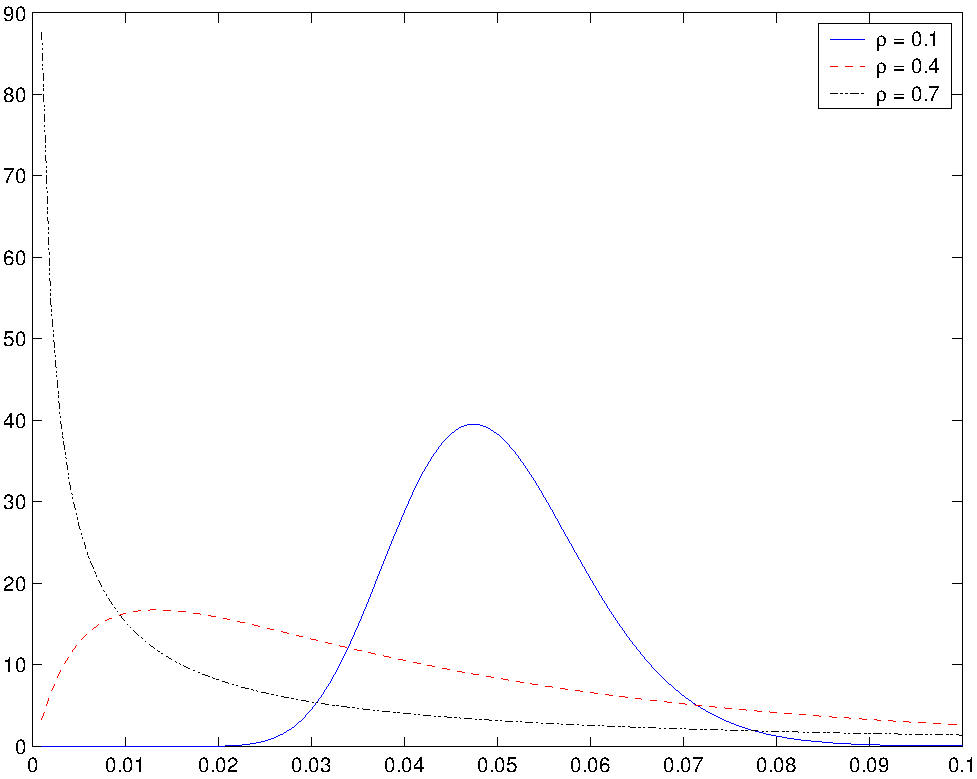
\includegraphics[width=0.8\textwidth]{./Figures/dens.pdf}
\caption{The density function $f$ as given in \eqref{density} for
  three different $\rho$'s and $\bar{p} = 0.05$. (Plotted on $[0,
  0.1]$ for convenience.)}
\label{fig:dens2}
\end{center}
\end{figure}


Let's see one more result on Table~\ref{tab:data}. According to~\cite{Fraz06}\ldots

% Table generated by Excel2LaTeX from sheet 'Sheet1'
\begin{table}
\caption{These are the data.} \label{tab:data}
\begin{center}
\begin{tabular}{l|rrrrrl}
\hline \hline
DJ CDX Tranches: &      0-3\% &      3-7\% &     7-10\% &    10-15\% &    15-30\% &       RMSE \\

Market mid spread &    40.00\% &      312.5 &      122.5 &       42.5 &       12.5 &            \\

Bid/Ask Spread &     2.00\% &         15.0 &          7 &          7 &          3 &            \\

Stochastic vol intensities &    41.80\% &      308.9 &      116.2 &       44.9 &          2 &       1.68 \\

Jump-diffusion intensities &    46.90\% &      340.2 &      119.7 &       61.9 &       14.3 &       2.17 \\

Pure-diffusion intensities &    49.30\% &      442.9 &       94.9 &       16.8 &        0.4 &       5.34 \\

Gaussian copula &    46.80\% &      474.4 &      131.8 &       36.9 &        2.9 &        5.3 \\

RFL Gaussian copula &    48.60\% &      334.9 &      125.5 &       66.5 &        9.2 &       2.59 \\

Double-t copula &    45.10\% &        367 &      114.9 &       54.9 &         20 &       2.44 \\
\hline \hline
\multicolumn{ 6}{l}{Source: Some source that I quote in the form Author (YYYY).} &

\end{tabular}
\end{center}
\end{table} 


\appendix
\chapter{Code}
%% Code file
\section{Java}
\subsection{CreateGrid.java}
\begin{verbatim}
import java.awt.*;

import java.sql.Connection;
import java.sql.DriverManager;
import java.sql.PreparedStatement;
import java.sql.SQLException;

import java.awt.geom.*;
import java.util.*;
import java.io.*;

/**
 * Created by Tharald Fongaard and Jacob Perricone on 10/02/15.
 */
public class CreateGrid {
    private SeparateChainingHashST<String,SeparateChainingHashST<Double,Pixelization>> pixels;
    private XMLReader xmlReader;
    private SeparateChainingHashST<Double,String> keyState;

    public CreateGrid() throws ClassNotFoundException, SQLException {
        xmlReader = new XMLReader();
        pixels = new SeparateChainingHashST<String, SeparateChainingHashST<Double, Pixelization>>();
        keyState = new SeparateChainingHashST<Double, String>();

        for(String state: xmlReader.getAllStates()){
            SeparateChainingHashST<Double,Pixelization> stateTable = new SeparateChainingHashST<Double, Pixelization>();
            pixels.put(state,stateTable);
        }

        int iStart;
        int iEnd;
        int jStart;
        int jEnd;

        double initiallat = 24.544091;
        double initallon = -120.5;
        double finallon = -106.25;
        double finallat = 48.987386;

        iStart = (int) Math.floor(138.348*(initallon + 97.5)*Math.cos(Math.toRadians(initiallat)));
        jStart = (int) Math.floor(138.348*(initiallat - 37.0));
        iEnd = (int) Math.floor(138.348*(finallon + 97.5)*Math.cos(Math.toRadians(finallat)));
        jEnd = (int) Math.floor(138.348*(finallat - 37.0));

        String url = "jdbc:mysql://127.0.0.1:3306/Grid";

        for(int i = iEnd; i >= iStart; i--){
            Class.forName("com.mysql.jdbc.Driver");
            Connection m_Connection = DriverManager.getConnection(url, "tharald", "putin");
            StdOut.println("" + i + " / " + iEnd);
            for(int j = jStart; j <= jEnd; j++){
                Pixelization pixel = new Pixelization(i,j);
                double key = pixel.get_id();
                Point2D cent = pixel.get_centroid();
                String state = xmlReader.getClosestState(cent);

                Point2D bl = pixel.get_bl();
                Point2D br = pixel.get_br();
                Point2D tr = pixel.get_tr();
                Point2D tl = pixel.get_tl();
                int x = i;
                int y = j;

                PreparedStatement total = m_Connection.prepareStatement("REPLACE INTO "+ state + " VALUES(?,?,?,?,?,?,?,?,?,?,?,?,?)");

                //ID
                total.setDouble(1, key);

                //X/Y
                total.setInt(2, x);
                total.setInt(3, y);

                //Centroid Long/Lat
                total.setDouble(4, cent.x());
                total.setDouble(5, cent.y());

                //Bottom Left Long/Lat
                total.setDouble(6, bl.x());
                total.setDouble(7, bl.y());

                //Bottom Right Long/Lat
                total.setDouble(8, br.x());
                total.setDouble(9, br.y());

                //Top Left Long/Lat
                total.setDouble(10, tl.x());
                total.setDouble(11, tl.y());

                //Top Right Long/Lat
                total.setDouble(12, tr.x());
                total.setDouble(13, tr.y());

                total.executeUpdate();
            }
            m_Connection.close();
        }


    }

    public Iterable<String> getStates(){
        return pixels.keys();
    }



    public double Size(){
        return pixels.size();
    }

    public Iterable<Double> getKeys(String state){
        return pixels.get(state).keys();
    }

    public int getX(double key){
        String state = keyState.get(key);
        Pixelization pixel = pixels.get(state).get(key);
        return pixel.get_x();
    }

    public int getY(double key){
        String state = keyState.get(key);
        Pixelization pixel = pixels.get(state).get(key);
        return pixel.get_y();
    }

    public Point2D getPixelCentroid(double key){
        String state = keyState.get(key);
        Pixelization pixel = pixels.get(state).get(key);
        Point2D returnPoint = pixel.get_centroid();
        return returnPoint;
    }

    public Point2D getPixelBr(double key){
        String state = keyState.get(key);
        Pixelization pixel = pixels.get(state).get(key);
        Point2D returnPoint = pixel.get_br();
        return returnPoint;
    }

    public Point2D getPixelBl(double key){
        String state = keyState.get(key);
        Pixelization pixel = pixels.get(state).get(key);
        Point2D returnPoint = pixel.get_bl();
        return returnPoint;
    }

    public Point2D getPixelTr(double key){
        String state = keyState.get(key);
        Pixelization pixel = pixels.get(state).get(key);
        Point2D returnPoint = pixel.get_tr();
        return returnPoint;
    }

    public Point2D getPixelTl(double key){
        String state = keyState.get(key);
        Pixelization pixel = pixels.get(state).get(key);
        Point2D returnPoint = pixel.get_tl();
        return returnPoint;

    }

    public static void main(String[] args) {
        CreateGrid grid = null;
        try {
            grid = new CreateGrid();
        } catch (ClassNotFoundException e) {
            e.printStackTrace();
        } catch (SQLException e) {
            e.printStackTrace();
        }
        StdOut.println("Done");
    }


}
\end{verbatim}

\subsection{Pixelization.java}
\begin{verbatim}
import java.util.*;
import java.io.*;
import java.awt.*;
import java.lang.Math;

public class Pixelization {
		double id;
		int x;
		int y;
		double CENTERLON = -97.5;
		double CENTERLAT = 37;
		double YHEIGHT = 0.00722814;
		double XWIDTH =  0.00944344;
		Point2D bottomleft;
		Point2D bottomright;
		Point2D topleft;
		Point2D topright;
		Point2D centroid;

	public Pixelization(int x, int y) {
		this.x = x;
		this.y = y;
		this.id = createid(x, y);
		this.bottomleft = createbottomleft(x, y);
		this.bottomright = createbottomright(x,y);
		this.topleft = createtopleft(x,y);
		this.topright = createtopright(x,y);
		this.centroid = createcentroid();
	}
	private double createid(int a, int b) {
        double returnn = 0.5*(a+195593+b+1724)*(a+195593+b+1724+1)+b+1724;
       // StdOut.println(returnn);
        return returnn;
    }

	private Point2D createbottomleft(int i, int j) {
		double lon, lat;
		double cosangle = Math.cos(Math.toRadians(CENTERLAT + j*YHEIGHT));
		lon = (CENTERLON + (YHEIGHT*i)/cosangle);
		lat = (CENTERLAT + YHEIGHT*j);
		Point2D p = new Point2D(lon, lat);
		return p;
	}
	private Point2D createbottomright(int i, int j) {
		i++;
		double lon, lat;
		double cosangle = Math.cos(Math.toRadians(CENTERLAT + j*YHEIGHT));
		lon = (CENTERLON + (YHEIGHT*i)/cosangle);
		lat = (CENTERLAT + YHEIGHT*j);
		Point2D p = new Point2D(lon, lat);
		return p;
	}

	private Point2D createtopleft(int i, int j) {
		j++;
		double lon, lat;
		double cosangle = Math.cos(Math.toRadians(CENTERLAT + j*YHEIGHT));
		lon = (CENTERLON + (YHEIGHT*i)/cosangle);
		lat = (CENTERLAT + YHEIGHT*j);
		Point2D p = new Point2D(lon, lat);
		return p;
	}

	private Point2D createtopright(int i, int j) {
		j++;
		i++;
		double lon, lat;
		double cosangle = Math.cos(Math.toRadians(CENTERLAT + j*YHEIGHT));
		lon = (CENTERLON + (YHEIGHT*i)/cosangle);
		lat = (CENTERLAT + YHEIGHT*j);
		Point2D p = new Point2D(lon, lat);
		return p;
	}

	private Point2D createcentroid() {
		double lon, lat;
		lon = (bottomleft.x() + bottomright.x())/2;
		lat = (bottomleft.y() + topleft.y())/2;
		Point2D p = new Point2D(lon, lat);
		return p;
	}

	public Point2D get_br() {
		return bottomright;
	}

	public int get_x() {
		return x;
	}

	public int get_y() {
		return y;
	}

	public double get_id() {
		return id;
	}

	public Point2D get_bl() {
		return bottomleft;
	}

	public Point2D get_tl() {
		return topleft;
	}

	public Point2D get_tr() {
		return topright;
	}

    public Point2D get_centroid(){
        return centroid;
    }

    public static void main(String[] args) {
    	double lat = Double.parseDouble(args[0]);
    	double lon = Double.parseDouble(args[1]);

    	System.out.println("Starting lat: " + lat + " , Starting lon: " + lon);
    	Point2D p = new Point2D(0.9,1.9);
    	Pixelization pixel = new Pixelization(lat, lon, p);
    	System.out.println("Lat : " + pixel.get_brLat() + "Long + " + pixel.get_brLong());

    }
}
\end{verbatim}
\subsection{Polygon.java}
\begin{verbatim}
import java.awt.*;

/*************************************************************************
 *  Compilation:  javac Polygon.java
 *  Execution:    java Polygon
 *  Dependencies: Point2D.java
 *
 *  Implementation of 2D polygon, possibly intersecting.
 *
 *
 *  Original Obtained from Princeton University algs4 library
 *  This version has been altered from the original
 *************************************************************************/

public class Polygon {
    private int N;        // number of points in the polygon
    private Point2D[] a;    // the points, setting points[0] = points[N]
    private String name;
    private Color color;

    // default buffer = 4
    public Polygon(String state, String colour) {
        N = 0;
        a = new Point2D[4];
        name = state;
        color = Color.decode(colour);

    }


    // double size of array
    private void resize() {
        Point2D[] temp = new Point2D[2*N+1];
        for (int i = 0; i <= N; i++) temp[i] = a[i];
        a = temp;
    }

    // return size
    public int size() { return N; }

    // draw polygon
    public void draw() {
        for (int i = 0; i < N; i++)
            a[i].drawTo(a[i+1]);
    }


    // add point p to end of polygon
    public void add(Point2D p) {
        if (N >= a.length - 1) resize();   // resize array if needed
        a[N++] = p;                        // add point
        a[N] = a[0];                       // close polygon
    }

    // return the perimeter
    public double perimeter() {
        double sum = 0.0;
        for (int i = 0; i < N; i++)
            sum = sum + a[i].distanceTo(a[i+1]);
        return sum;
    }

    public Iterable<Point2D> getAll(){
        Stack<Point2D> stack = new Stack<Point2D>();
        for (int i = 0; i < N; i++){
            stack.push(a[i]);
        }
        return stack;

    }

    // return signed area of polygon
    public double area() {
        double sum = 0.0;
        for (int i = 0; i < N; i++) {
            sum = sum + (a[i].x() * a[i+1].y()) - (a[i].y() * a[i+1].x());
        }
        return 0.5 * sum;
    }

    // does this Polygon contain the point p?
    // if p is on boundary then 0 or 1 is returned, and p is in exactly one point of every partition of plane
    // Reference: http://exaflop.org/docs/cgafaq/cga2.html
    public boolean contains2(Point2D p) {
        int crossings = 0;
        for (int i = 0; i < N; i++) {
            int j = i + 1;
            boolean cond1 = (a[i].y() <= p.y()) && (p.y() < a[j].y());
            boolean cond2 = (a[j].y() <= p.y()) && (p.y() < a[i].y());
            if (cond1 || cond2) {
                // need to cast to double
                if (p.x() < (a[j].x() - a[i].x()) * (p.y() - a[i].y()) / (a[j].y() - a[i].y()) + a[i].x())
                    crossings++;
            }
        }
        if (crossings % 2 == 1) return true;
        else                    return false;
    }

    // does this Polygon contain the point p?
    // Reference: http://softsurfer.com/Archive/algorithm_0103/algorithm_0103.htm
    public boolean contains(Point2D p) {
        int winding = 0;
        for (int i = 0; i < N; i++) {
            int ccw = Point2D.ccw(a[i], a[i+1], p);
            if (a[i+1].y() >  p.y() && p.y() >= a[i].y())  // upward crossing
                if (ccw == +1) winding++;
            if (a[i+1].y() <= p.y() && p.y() <  a[i].y())  // downward crossing
                if (ccw == -1) winding--;
        }
        return winding != 0;
    }


    // return string representation of this point
    public String toString() {
        if (N == 0) return "[ ]";
        String s = "";
        s = s + "[ ";
        for (int i = 0; i <= N; i++)
            s = s + a[i] + " ";
        s = s + "]";
        return s;
    }

    public String getName(){
        return name;
    }

    public Point2D centroid(){
        double cX = 0;
        double cY = 0;
        for (int i = 0; i <= N; i++){
            cX = cX + a[i].x();
            cY = cY + a[i].y();
        }
        cX = cX/N;
        cY = cY/N;
        Point2D rPoint =new Point2D(cX,cY);
        return rPoint;
    }

    public Color color(){
        return color;
    }


    // test client
    public static void main(String[] args) {
        int N = 10;

        // a square
        Polygon poly = new Polygon("STATE", "#ff0000");
        poly.add(new Point2D(5, 5));
        poly.add(new Point2D(9, 5));
        poly.add(new Point2D(9, 9));
        poly.add(new Point2D(5, 9));

        System.out.println("polygon    = " + poly);
        System.out.println("perimeter  = " + poly.perimeter());
        System.out.println("area       = " + poly.area());

        System.out.println("contains(5, 5) = " + poly.contains(new Point2D(5, 5)));
        System.out.println("contains(9, 5) = " + poly.contains(new Point2D(9, 5)));
        System.out.println("contains(9, 9) = " + poly.contains(new Point2D(9, 9)));
        System.out.println("contains(5, 9) = " + poly.contains(new Point2D(5, 9)));
        System.out.println("contains(7, 5) = " + poly.contains(new Point2D(7, 5)));
        System.out.println("contains(5, 7) = " + poly.contains(new Point2D(5, 7)));
        System.out.println("contains(7, 9) = " + poly.contains(new Point2D(7, 9)));
        System.out.println("contains(9, 7) = " + poly.contains(new Point2D(9, 7)));

        // generate N random points in the unit square and check what fraction are in the polygon
        int yes = 0;
        for (int i = 0; i < N; i++) {
            int x = (int) (10 * Math.random());
            int y = (int) (10 * Math.random());
            Point2D p = new Point2D(x, y);
            if (poly.contains(p)) yes++;
            if (poly.contains(p) != poly.contains2(p)) System.out.println("different " + p);
        }

        // true answer is = 0.16 (depends on how boundary points are handled)
        System.out.println("Fraction in polygon = " + 1.0 * yes / N);


    }
}
\end{verbatim}
\subsection{XMLreader.java}
\begin{verbatim}
import jdk.internal.org.xml.sax.SAXException;
import org.w3c.dom.Document;
import org.w3c.dom.*;



import javax.xml.parsers.DocumentBuilder;
import javax.xml.parsers.DocumentBuilderFactory;
import javax.xml.parsers.ParserConfigurationException;
import java.awt.*;
import java.io.IOException;


/**
 * Created by Tharald on 17/02/15.
 */
public class XMLReader {
    private KdTreeST<Polygon> treeST;
    private SeparateChainingHashST<String,Polygon> states;


    public XMLReader(){
        treeST = new KdTreeST<Polygon>();
        states = new SeparateChainingHashST<String, Polygon>();

        DocumentBuilderFactory builderFactory = DocumentBuilderFactory.newInstance();

        try{
            DocumentBuilder dBuilder = builderFactory.newDocumentBuilder();
            Document document = dBuilder.parse(XMLReader.class.getResourceAsStream("/states.xml"));
            Document centroidsDocument = dBuilder.parse(XMLReader.class.getResourceAsStream("/centroids.xml"));
            document.normalize();
            centroidsDocument.normalize();

            NodeList centroids = centroidsDocument.getElementsByTagName("states");
            Node centroidRoot = centroids.item(0);
            Element centroidElementRoot = (Element) centroidRoot;

            NodeList rootNodes = document.getElementsByTagName("states");
            org.w3c.dom.Node rootNode = rootNodes.item(0);
            org.w3c.dom.Element rootElement = (org.w3c.dom.Element) rootNode;

            NodeList statesList = rootElement.getElementsByTagName("state");
            NodeList centroidList = centroidElementRoot.getElementsByTagName("state");

            for(int i = 0; i < statesList.getLength();i++){
                org.w3c.dom.Node theState = statesList.item(i);
                org.w3c.dom.Element stateElement = (org.w3c.dom.Element) theState;
                //StdOut.println("This state is " + stateElement.getAttribute("name"));
                Polygon newState = new Polygon(stateElement.getAttribute("name"), stateElement.getAttribute("colour"));

                NodeList pointList = stateElement.getElementsByTagName("point");
                for(int j = 0; j < pointList.getLength();j++){
                    org.w3c.dom.Element pointElement = (org.w3c.dom.Element) pointList.item(j);
                    Point2D newPoint = new Point2D(Double.parseDouble(pointElement.getAttribute("lng")),Double.parseDouble(pointElement.getAttribute("lat")));
                    newState.add(newPoint);
                    //StdOut.println("Lat: " + pointElement.getAttribute("lat") + "Long: " + pointElement.getAttribute("lng"));
                }
                Node statecentroid = centroidList.item(i);
                Element centroidElement = (Element) statecentroid;
                Point2D centroid = new Point2D(Double.parseDouble(centroidElement.getAttribute("lon")),Double.parseDouble(centroidElement.getAttribute("lat")));
                treeST.insert(centroid,newState);
                states.put(stateElement.getAttribute("name"),newState);

            }
            Polygon nostate = new Polygon("NoState","#ff0000");
            states.put("NoState", nostate);


        }
        catch (ParserConfigurationException e){
            e.printStackTrace();
        }
        catch (org.xml.sax.SAXException e){
            e.printStackTrace();
        }
        catch (IOException e){
            e.printStackTrace();
        }
    }

    public Polygon getStatePolygon(String state){
        return states.get(state);
    }

    public Iterable<Polygon> getAllPolygons(){
        return treeST.getAllValues();
    }

    public String getClosestState(Point2D queryPoint){
        Point2D nearestPoint = treeST.nearest(queryPoint);
        Polygon nearestState = treeST.get(nearestPoint);
        if(nearestState.contains(queryPoint)){
            return nearestState.getName();
        }
        else{
            for(Polygon pol:treeST.getAllValues()){
                if(pol.contains(queryPoint)){
                    return pol.getName();
                }
            }
        }
        return "NoState";
    }

    public int size(){
        return treeST.size();
    }

    public Iterable<String> getAllStates() {
        return states.keys();

    }

    public Iterable<Point2D> getAllPoints(){
        return treeST.getAllPoints();
    }
    public void drawTree(){
        treeST.draw();
    }



    public static void main(String[] args){
       XMLReader xmlReader = new XMLReader();
        StdOut.println(xmlReader.size());
        StdDraw.setXscale(-136,-66);
        StdDraw.setYscale(20.54,53);
        /*for(String s: xmlReader.getAllStates()){
            StdOut.println(s);
        }

        StdDraw.setPenColor(Color.GREEN);
        int points= 0;
        for(Point2D p:xmlReader.getAllPoints()){
            p.draw();
            points++;
        }
        */
        for(Polygon p:xmlReader.getAllPolygons()){
            StdDraw.setPenColor(p.color());
            p.draw();
        }
        //StdOut.println(points);
        //xmlReader.drawTree();
        StdDraw.setPenColor(Color.BLACK);
        StdDraw.setPenRadius(.006);

        for(Point2D p:xmlReader.getAllPoints()){
            p.draw();
        }

    }
}
\end{verbatim}
\subsection{TestFrame.java}
\begin{verbatim}
/**
 * Created by Tharald on 22/02/15.
 */

import org.openstreetmap.gui.jmapviewer.*;
import org.openstreetmap.gui.jmapviewer.events.JMVCommandEvent;
import org.openstreetmap.gui.jmapviewer.interfaces.*;
import org.openstreetmap.gui.jmapviewer.tilesources.BingAerialTileSource;
import org.openstreetmap.gui.jmapviewer.tilesources.MapQuestOpenAerialTileSource;
import org.openstreetmap.gui.jmapviewer.tilesources.MapQuestOsmTileSource;
import org.openstreetmap.gui.jmapviewer.tilesources.OsmTileSource;

import java.awt.*;
import java.awt.Point;
import java.awt.event.ActionEvent;
import java.awt.event.ActionListener;
import java.awt.event.ItemEvent;
import java.awt.event.ItemListener;
import java.awt.event.MouseAdapter;
import java.awt.event.MouseEvent;
import java.io.IOException;
import java.sql.*;
import java.util.*;
import java.util.List;

import javax.swing.JButton;
import javax.swing.JCheckBox;
import javax.swing.JComboBox;
import javax.swing.JFrame;
import javax.swing.JLabel;
import javax.swing.JPanel;

public class TestFrame extends JFrame implements JMapViewerEventListener {

    private static final long serialVersionUID = 1L;

    private JMapViewerTree treeMap = null;

    private JLabel zoomLabel=null;
    private JLabel zoomValue=null;

    private JLabel mperpLabelName=null;
    private JLabel mperpLabelValue = null;

    public TestFrame() {

        super("TrafficFlow");
        XMLReader xmlreader = new XMLReader();
        setSize(400, 400);

        treeMap = new JMapViewerTree("Zones");

        // Listen to the map viewer for user operations so components will
        // recieve events and update
        map().addJMVListener(this);

        // final JMapViewer map = new JMapViewer(new MemoryTileCache(),4);
        // map.setTileLoader(new OsmFileCacheTileLoader(map));
        // new DefaultMapController(map);

        setLayout(new BorderLayout());
        setDefaultCloseOperation(JFrame.EXIT_ON_CLOSE);
        setExtendedState(JFrame.MAXIMIZED_BOTH);
        JPanel panel = new JPanel();
        JPanel panelTop = new JPanel();
        JPanel panelBottom = new JPanel();
        JPanel helpPanel = new JPanel();
        JPanel sqlPanel = new JPanel();




        mperpLabelName=new JLabel("Meters/Pixels: ");
        mperpLabelValue=new JLabel(String.format("%s",map().getMeterPerPixel()));

        zoomLabel=new JLabel("Zoom: ");
        zoomValue=new JLabel(String.format("%s", map().getZoom()));

        add(panel, BorderLayout.NORTH);
        add(helpPanel, BorderLayout.SOUTH);
        panel.setLayout(new BorderLayout());
        panel.add(panelTop, BorderLayout.NORTH);
        panel.add(panelBottom, BorderLayout.SOUTH);
        add(sqlPanel,BorderLayout.EAST);
        JLabel helpLabel = new JLabel("Use right mouse button to move,\n "
                + "left double click or mouse wheel to zoom.");
        helpPanel.add(helpLabel);
        JButton button = new JButton("setDisplayToFitMapMarkers");
        button.addActionListener(new ActionListener() {

            public void actionPerformed(ActionEvent e) {
                map().setDisplayToFitMapMarkers();
            }
        });
        JComboBox<TileSource> tileSourceSelector = new JComboBox<>(new TileSource[] { new OsmTileSource.Mapnik(),
                new OsmTileSource.CycleMap(), new BingAerialTileSource(), new MapQuestOsmTileSource(), new MapQuestOpenAerialTileSource() });
        tileSourceSelector.addItemListener(new ItemListener() {
            public void itemStateChanged(ItemEvent e) {
                map().setTileSource((TileSource) e.getItem());
            }
        });
        JComboBox<TileLoader> tileLoaderSelector;
        try {
            tileLoaderSelector = new JComboBox<>(new TileLoader[] { new OsmFileCacheTileLoader(map()), new OsmTileLoader(map()) });
        } catch (IOException e) {
            tileLoaderSelector = new JComboBox<>(new TileLoader[] { new OsmTileLoader(map()) });
        }
        tileLoaderSelector.addItemListener(new ItemListener() {
            public void itemStateChanged(ItemEvent e) {
                map().setTileLoader((TileLoader) e.getItem());
            }
        });
        map().setTileLoader((TileLoader) tileLoaderSelector.getSelectedItem());
        panelTop.add(tileSourceSelector);
        panelTop.add(tileLoaderSelector);
        final JCheckBox showMapMarker = new JCheckBox("Map markers visible");
        showMapMarker.setSelected(map().getMapMarkersVisible());
        showMapMarker.addActionListener(new ActionListener() {
            public void actionPerformed(ActionEvent e) {
                map().setMapMarkerVisible(showMapMarker.isSelected());
            }
        });
        panelBottom.add(showMapMarker);
        ///
        final JCheckBox showTreeLayers = new JCheckBox("Tree Layers visible");
        showTreeLayers.addActionListener(new ActionListener() {
            public void actionPerformed(ActionEvent e) {
                treeMap.setTreeVisible(showTreeLayers.isSelected());
            }
        });
        panelBottom.add(showTreeLayers);
        ///
        final JCheckBox showToolTip = new JCheckBox("ToolTip visible");
        showToolTip.addActionListener(new ActionListener() {
            public void actionPerformed(ActionEvent e) {
                map().setToolTipText(null);
            }
        });
        panelBottom.add(showToolTip);
        ///
        final JCheckBox showTileGrid = new JCheckBox("Tile grid visible");
        showTileGrid.setSelected(map().isTileGridVisible());
        showTileGrid.addActionListener(new ActionListener() {
            public void actionPerformed(ActionEvent e) {
                map().setTileGridVisible(showTileGrid.isSelected());
            }
        });
        panelBottom.add(showTileGrid);
        final JCheckBox showZoomControls = new JCheckBox("Show zoom controls");
        showZoomControls.setSelected(map().getZoomContolsVisible());
        showZoomControls.addActionListener(new ActionListener() {
            public void actionPerformed(ActionEvent e) {
                map().setZoomContolsVisible(showZoomControls.isSelected());
            }
        });
        panelBottom.add(showZoomControls);
        final JCheckBox scrollWrapEnabled = new JCheckBox("Scrollwrap enabled");
        scrollWrapEnabled.addActionListener(new ActionListener() {
            public void actionPerformed(ActionEvent e) {
                map().setScrollWrapEnabled(scrollWrapEnabled.isSelected());
            }
        });
        panelBottom.add(scrollWrapEnabled);
        panelBottom.add(button);

        panelTop.add(zoomLabel);
        panelTop.add(zoomValue);
        panelTop.add(mperpLabelName);
        panelTop.add(mperpLabelValue);

        add(treeMap, BorderLayout.CENTER);

        //

        LayerGroup pixelGroup = new LayerGroup("States");
        pixelGroup.setVisible(true);
        SeparateChainingHashST<String, Layer>  states = new SeparateChainingHashST<String,Layer>();


        String[] options = new String[51];
        int i = 0;
        for(String s: xmlreader.getAllStates()) {
            Layer layer = pixelGroup.addLayer(s);
           states.put(s,layer);
           Polygon pol = xmlreader.getStatePolygon(s);

            List<Coordinate> list = new ArrayList<Coordinate>();
            for(Point2D p: pol.getAll()){
                list.add(c(p));
            }


            MapPolygon thisState = new MapPolygonImpl(layer,s,list);
            map().addMapPolygon(thisState);
            treeMap.addLayer(layer);
            options[i] = s;
            i++;


        }
        JComboBox jComboBox = new JComboBox(options);

       sqlPanel.add(jComboBox);

        JButton getPixels = new JButton();
        getPixels.addActionListener(new ActionListener() {

            public void actionPerformed(ActionEvent e) {
                try {
                    Class.forName("com.mysql.jdbc.Driver");
                } catch (ClassNotFoundException e1) {
                    e1.printStackTrace();
                }
                String url = "jdbc:mysql://127.0.0.1:3306/Grid";
                try {
                    Connection m_Connection = DriverManager.getConnection(url, "tharald", "putin");
                    PreparedStatement total = m_Connection.prepareStatement("SELECT * FROM " + jComboBox.getSelectedItem());
                    ResultSet resultSet = total.executeQuery();
                   while(resultSet.next()){
                       double bl_long = resultSet.getDouble(6);
                       double bl_lat = resultSet.getDouble(7);
                       double br_long = resultSet.getDouble(8);
                       double br_lat = resultSet.getDouble(9);
                       double tl_long = resultSet.getDouble(10);
                       double tl_lat = resultSet.getDouble(11);
                       double tr_long = resultSet.getDouble(12);
                       double tr_lat = resultSet.getDouble(13);
                       String state = (String) jComboBox.getSelectedItem();
                       List<Coordinate> points = new ArrayList<Coordinate>();
                       points.add(c(bl_lat, bl_long));
                       points.add(c(br_lat,br_long));
                       points.add(c(tr_lat,tr_long));
                       points.add(c(tl_lat,tl_long));


                       MapPolygonImpl  pix =  new MapPolygonImpl(states.get(state),points);
                       map().addMapPolygon(pix);

                   }



                } catch (SQLException e1) {
                    e1.printStackTrace();
                }
                //StdOut.println("Connection Successful");


            }
        });

        sqlPanel.add(getPixels);




        // map.setDisplayPosition(new Coordinate(49.807, 8.6), 11);
        // map.setTileGridVisible(true);

        map().addMouseListener(new MouseAdapter() {
            @Override
            public void mouseClicked(MouseEvent e) {
                if (e.getButton() == MouseEvent.BUTTON1) {
                    map().getAttribution().handleAttribution(e.getPoint(), true);
                }
            }
        });

        map().addMouseMotionListener(new MouseAdapter() {
            @Override
            public void mouseMoved(MouseEvent e) {
                Point p = e.getPoint();
                boolean cursorHand = map().getAttribution().handleAttributionCursor(p);
                if (cursorHand) {
                    map().setCursor(new Cursor(Cursor.HAND_CURSOR));
                } else {
                    map().setCursor(new Cursor(Cursor.DEFAULT_CURSOR));
                }
                if(showToolTip.isSelected()) map().setToolTipText(map().getPosition(p).toString());
            }
        });
    }

    @Override
    public void processCommand(JMVCommandEvent command) {
        if (command.getCommand().equals(JMVCommandEvent.COMMAND.ZOOM) ||
                command.getCommand().equals(JMVCommandEvent.COMMAND.MOVE)) {
            updateZoomParameters();
        }
    }

    private void updateZoomParameters() {
        if (mperpLabelValue!=null)
            mperpLabelValue.setText(String.format("%s",map().getMeterPerPixel()));
        if (zoomValue!=null)
            zoomValue.setText(String.format("%s", map().getZoom()));
    }

    private JMapViewer map(){
        return treeMap.getViewer();
    }
    private static Coordinate c(double lat, double lon){
        return new Coordinate(lat, lon);
    }
    private static Coordinate c(Point2D p){
        return new Coordinate(p.y(),p.x());
    }


    public static void main(String[] args) {
        // java.util.Properties systemProperties = System.getProperties();
        // systemProperties.setProperty("http.proxyHost", "localhost");
        // systemProperties.setProperty("http.proxyPort", "8008");
        new TestFrame().setVisible(true);
    }
}
\end{verbatim}





\bibliographystyle{apa}
\bibliography{./Bibliography/refs} \label{bib}
\end{document}
